
\documentclass[preprint,12pt]{elsarticle}

\usepackage[spanish]{babel}
\usepackage{amssymb}
\usepackage{graphicx}
\usepackage{lineno}
\usepackage[utf8]{inputenc}
\usepackage{url}
\usepackage{natbib} 
\usepackage{amsmath} 
\usepackage{amssymb} 

\begin{document}
	
	\begin{frontmatter}

		\title{\huge DevOps en Base de Datos}
		
		\author{Estrella Palacios, Katherine Lizbeth              	(2016056193))}
		\author{Gonzales Cave, Angel Gabriel              	(xxxxxxxxxx))} %%cambiar
		\author{Huichi Contreras, Franklin Carlos         	(2016054948))} %%cambiar
		\author{Huillca Umpiri, Willian Arturo             		(xxxxxxxxxx))} %%cambiar 
		\address{Tacna, Perú}
		
%% ABSTRACT --------------------------------------------------------------------------------------------------------------------

		\begin{abstract}
		
EDITAR

		\end{abstract}

%% ----------------------------------------------------------------------------------------------------------------------------------

	\end{frontmatter}

%% RESUMEN ---------------------------------------------------------------------------------------------------------------------

	\section{Resumen}

Devops es describido como una relación cooperativa y productiva entre los equipos de desarrollo y los equipos de operación. Es por ello que DevOps logra establecer una relación eficaz, de eficiencia, colaboración y estrategias de desarrollo entre los colaboradores.
El concepto nace de una abreviatura de Dev como developers y Ops como operations (definidos en inglés), estableciendo como la idea principal el romper la barrera entre los mismos. 
DevOps también adopta nuevas metodologías de desarrollo como el desarrollo ágil, operaciones, control de calidad e implementación con el fin de crear integración y colaboración entre los dos departamentos.
En conclusión, la comunicación y colaboración entre los departamentos de desarrolladores y operaciones hacen de esta metodología la mejor opción para recurrir a un modelo de trabajo ordenado y bien estructurado.

%% ----------------------------------------------------------------------------------------------------------------------------------


%% INTRODUCION ----------------------------------------------------------------------------------------------------------------

\section{Introducción} 

EDITAR

\begin{itemize}
\item A
\item B
\item C


\end{itemize}

%% ----------------------------------------------------------------------------------------------------------------------------------


%% MARCO TEÓRICO ------------------------------------------------------------------------------------------------------------

\section{Marco Teórico}

%% PRIMERA SUBSECCION 

\subsection {\textbf{A}}

\subsubsection{\textbf{A.1}}

EDITAR \cite{SQLne}  %% EJEMPLO DE COMO CITAR UNA REFERENCIA EN UN PÁRRAFO

\subsubsection{\textbf{A.2}}

EDITAR

\begin{figure}[htb]
	\begin{center}
		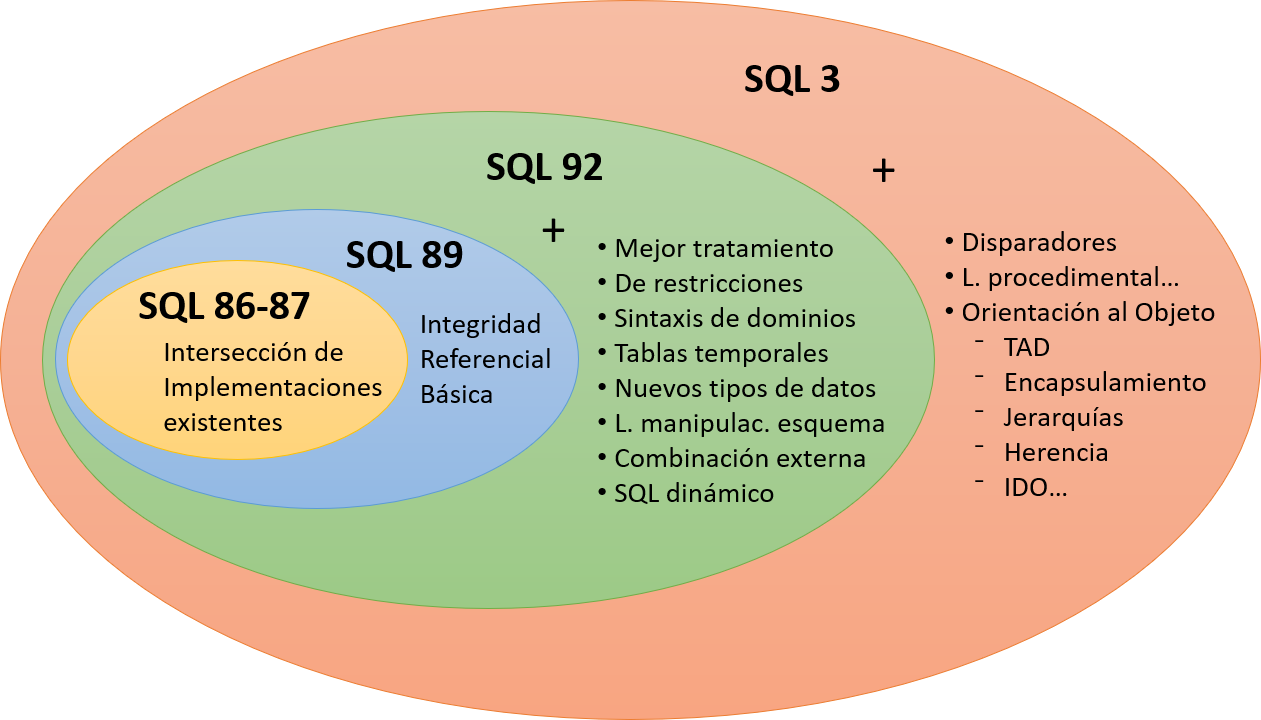
\includegraphics[width=10.5cm]{./IMAGENES/evolucion} %%EJEMPLO PARA INCLUIR IMAGEN
	\end{center}
\end{figure}


\subsubsection{\textbf{A.3}}

EDITAR

\begin{itemize}

\item x
\item y
\item z

\end{itemize}

%% SEGUNDA SUBSECCION

\subsection{\textbf{B}}

\subsubsection{\textbf{B.1}}

EDITAR

\subsubsection{\textbf{B.2}}	

EDITAR

\subsubsection{\textbf{B.3}}	

EDITAR


%% ----------------------------------------------------------------------------------------------------------------------------------


%% ANÁLISIS ( APLICACIÓN ) ---------------------------------------------------------------------------------------------------

\section{Análisis}

EDITAR

%% ----------------------------------------------------------------------------------------------------------------------------------


%% CONCLUSIONES ---------------------------------------------------------------------------------------------------------------

\section{Conclusiones}

\begin{itemize}

\item Conclusion 1 : \\ A

\item Conclusion 2 : \\ B

\item Conclusion 3 : \\ C

\end{itemize}

%% ----------------------------------------------------------------------------------------------------------------------------------

%%  REFERENCIAS BIBLIOGRÁFICAS ------------------------------------------------------------------------------------------
	
	\newpage
	
	\bibliographystyle{apalike} 	%ESTILO
	\bibliography{BIBLIOGRAFIA}	 
	
	
\end{document}
